\documentclass[a4paper,12pt]{article} % тип документа

\usepackage{biblatex}
\addbibresource{sample.bib}

%  Русский язык

\usepackage[T2A]{fontenc}			% кодировка
\usepackage[utf8]{inputenc}			% кодировка исходного текста
\usepackage[english,russian]{babel}	% локализация и переносы


% Математика
\usepackage{amsmath,amsfonts,amssymb,amsthm,mathtools, textcomp} 

% Графика
\usepackage{graphicx}

% Гиперссылки
\usepackage{hyperref}
\hypersetup{
    colorlinks=true,
    linkcolor=blue,
    filecolor=magenta,      
    urlcolor=cyan,
    pdftitle={Overleaf Example},
    pdfpagemode=FullScreen,
    }
 
\usepackage{caption}
\usepackage{wasysym}

%Заговолок
\author{Петросян Акоб}
\title{ МФТИ \\ ~ \\ ~ \\ Защита информации \\ ~ \\ Безопасная подводная связь на квантовом уровне }
\date{\today}


\begin{document} % начало документа

\maketitle
\newpage

\begin{figure}
  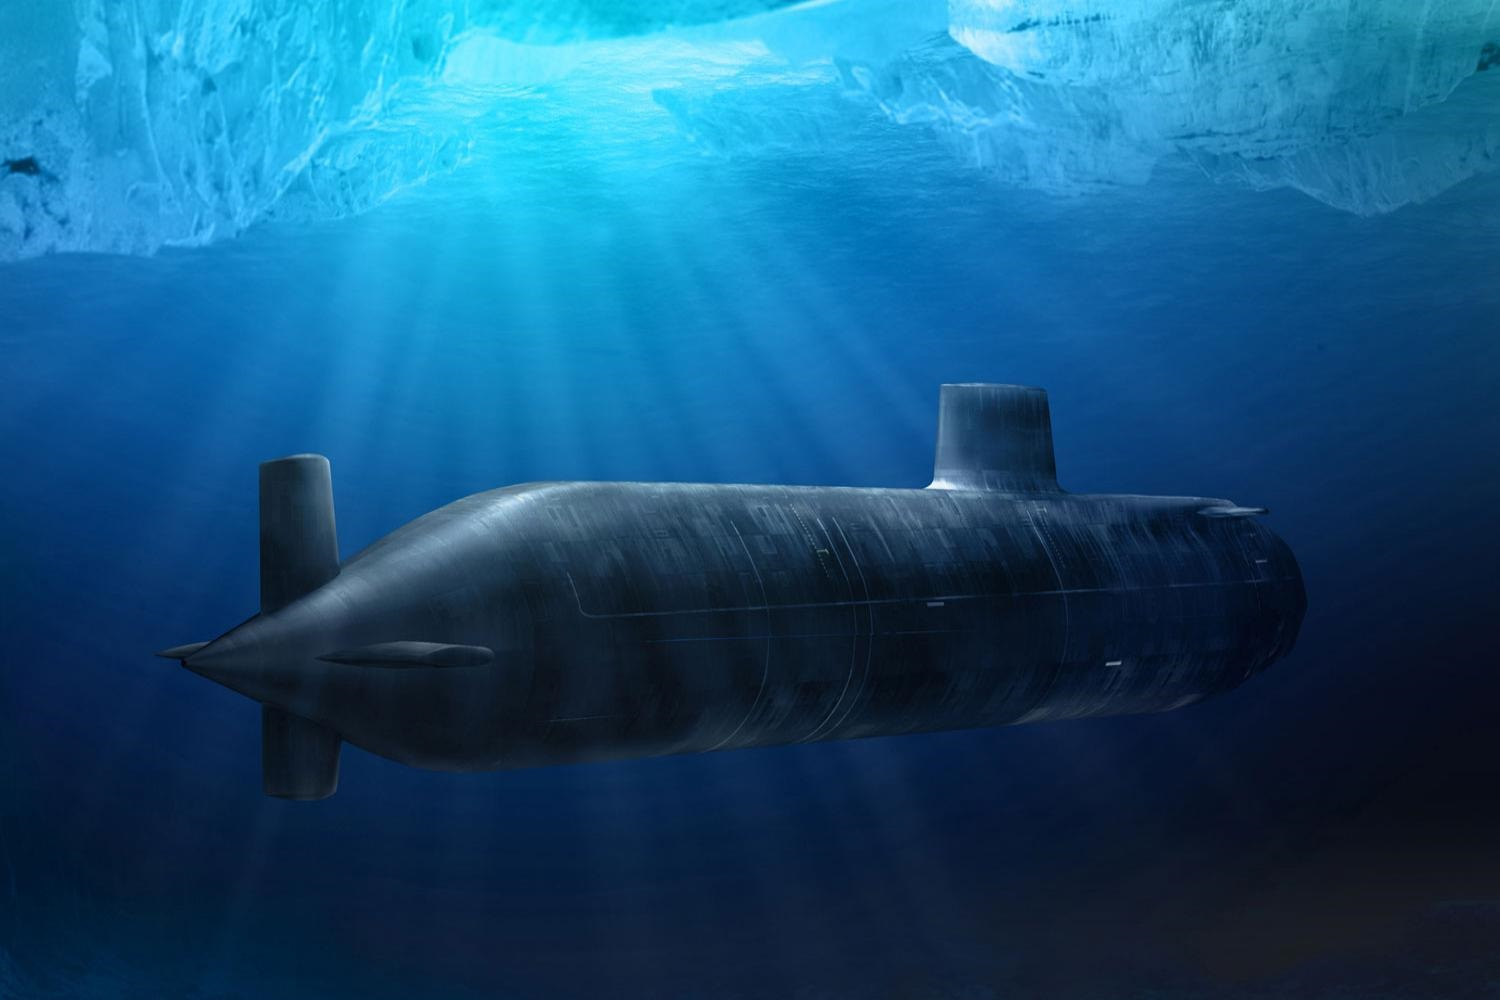
\includegraphics[width=\linewidth]{img/submarine.jpg}
  \captionof{figure}{Подводная лодка класса Astute Королевского флота является ударной подводной лодкой с ядерной установкой.}
  \label{fig:boat1}
\end{figure}

В этой обзорной статье рассмотрим некоторые из основных способов коммуникации подводных лодок. Изучим технологию квантового распределения ключей, которая позволяет подводным лодкам безопасно общаться как на глубине, так и на скорости.

\section*{Проблемы подводной связи}

\hspace{13pt} Чтобы оставаться не замеченной от гидролокаторов подводная лодка должна находиться на глубине от 60 до 100 метров. Но поддерживать подводную связь между подлодками или подлодками и базой довольно затруднительно, так как обычные радиоволны очень быстро поглощаются уже на глубине несколько десятков метров. Поэтому вместо "обычных" радиоволн используются волны с очень низкими или крайне низкими частотами(далее ОНЧ и КНЧ). Это волны, которые хорошо проникают вглубь воды, отражаются от ионосферы Земли и слабо поглощаются земной поверхностью.
~\\~

\noindent%
\begin{minipage}{\linewidth}% to keep image and caption on one page
\makebox[\linewidth]{%        to center the image
  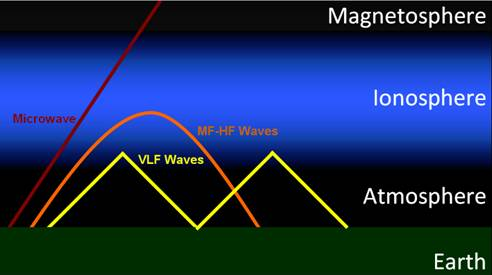
\includegraphics[keepaspectratio=true,scale=1]{img/elf_vlf.jpg}}
\captionof{figure}{ОНЧ волны}\label{SVM}%      only if needed  
\end{minipage}

~\\

Слабости такого подхода состоят в том, что чаще всего лодке надо буксировать огромные кабели-антены над водой, которых легко заметить с самолётов. Да и двигаться лодка может только с очень низкой скоростью, в определенном направлении.
~\\~

\noindent%
\begin{minipage}{\linewidth}% to keep image and caption on one page
\makebox[\linewidth]{%        to center the image
  \includegraphics[keepaspectratio=true,scale=0.35]{img/Towed_lens.png}}
\captionof{figure}{ОНЧ волны}\label{SVM}%      only if needed  
\end{minipage}

~\\

Хвастаться скоростью передачи такой метод тоже не может, так как ОНЧ и КНЧ предлагают только очень низкую полосу пропускания: ОНЧ поддерживает несколько сотен бит в секунду, а КНЧ - всего несколько бит в минуту.

Учитывая все эти недостатки, исследователи предлагают использовать технику под названием квантовое распределение ключей (КРК, {\it английский: QKD}), с помощью которой сумели добиться впечатляющих успехов не жертвуя скоростью и не заставляя подводную лодку подниматься ближе к поверхности. При этом безопасность связи гарантируется принципами квантовой механики. 

Что касается вида канала связи, ещё в 1980-х годах, были эксперименты, демонстрирующие способ поддержания оптического канала между подводной лодкой и воздушной платформой, используя оптическую связь с помощью лазера.

Группа Quantum Technologies из компании ITT Exelis, специализирующейся на оборонных технологиях, рассматривает возможность сделать еще один шаг вперед, исследуя возможность лазерной оптической связи между подводной лодкой и спутником или бортовой платформой, защищенной с помощью квантовой информации.

\section*{Квантовое распределение ключей(QKD)}

\hspace{13pt} Квантовое распределение ключей - это безопасный метод связи, реализующий криптографический протокол, включающий компоненты квантовой механики, который позволяет двум сторонам создать общий случайный секретный ключ, известный только им, который затем может использоваться для шифрования и дешифрования сообщений.

Единицей квантовой информации является кубит, который представляет собой квантовое состояние фотона. Это может быть ноль, единица или любая суперпозиция нуля и единицы.

~\\~

\noindent%
\begin{minipage}{\linewidth}% to keep image and caption on one page
\makebox[\linewidth]{%        to center the image
  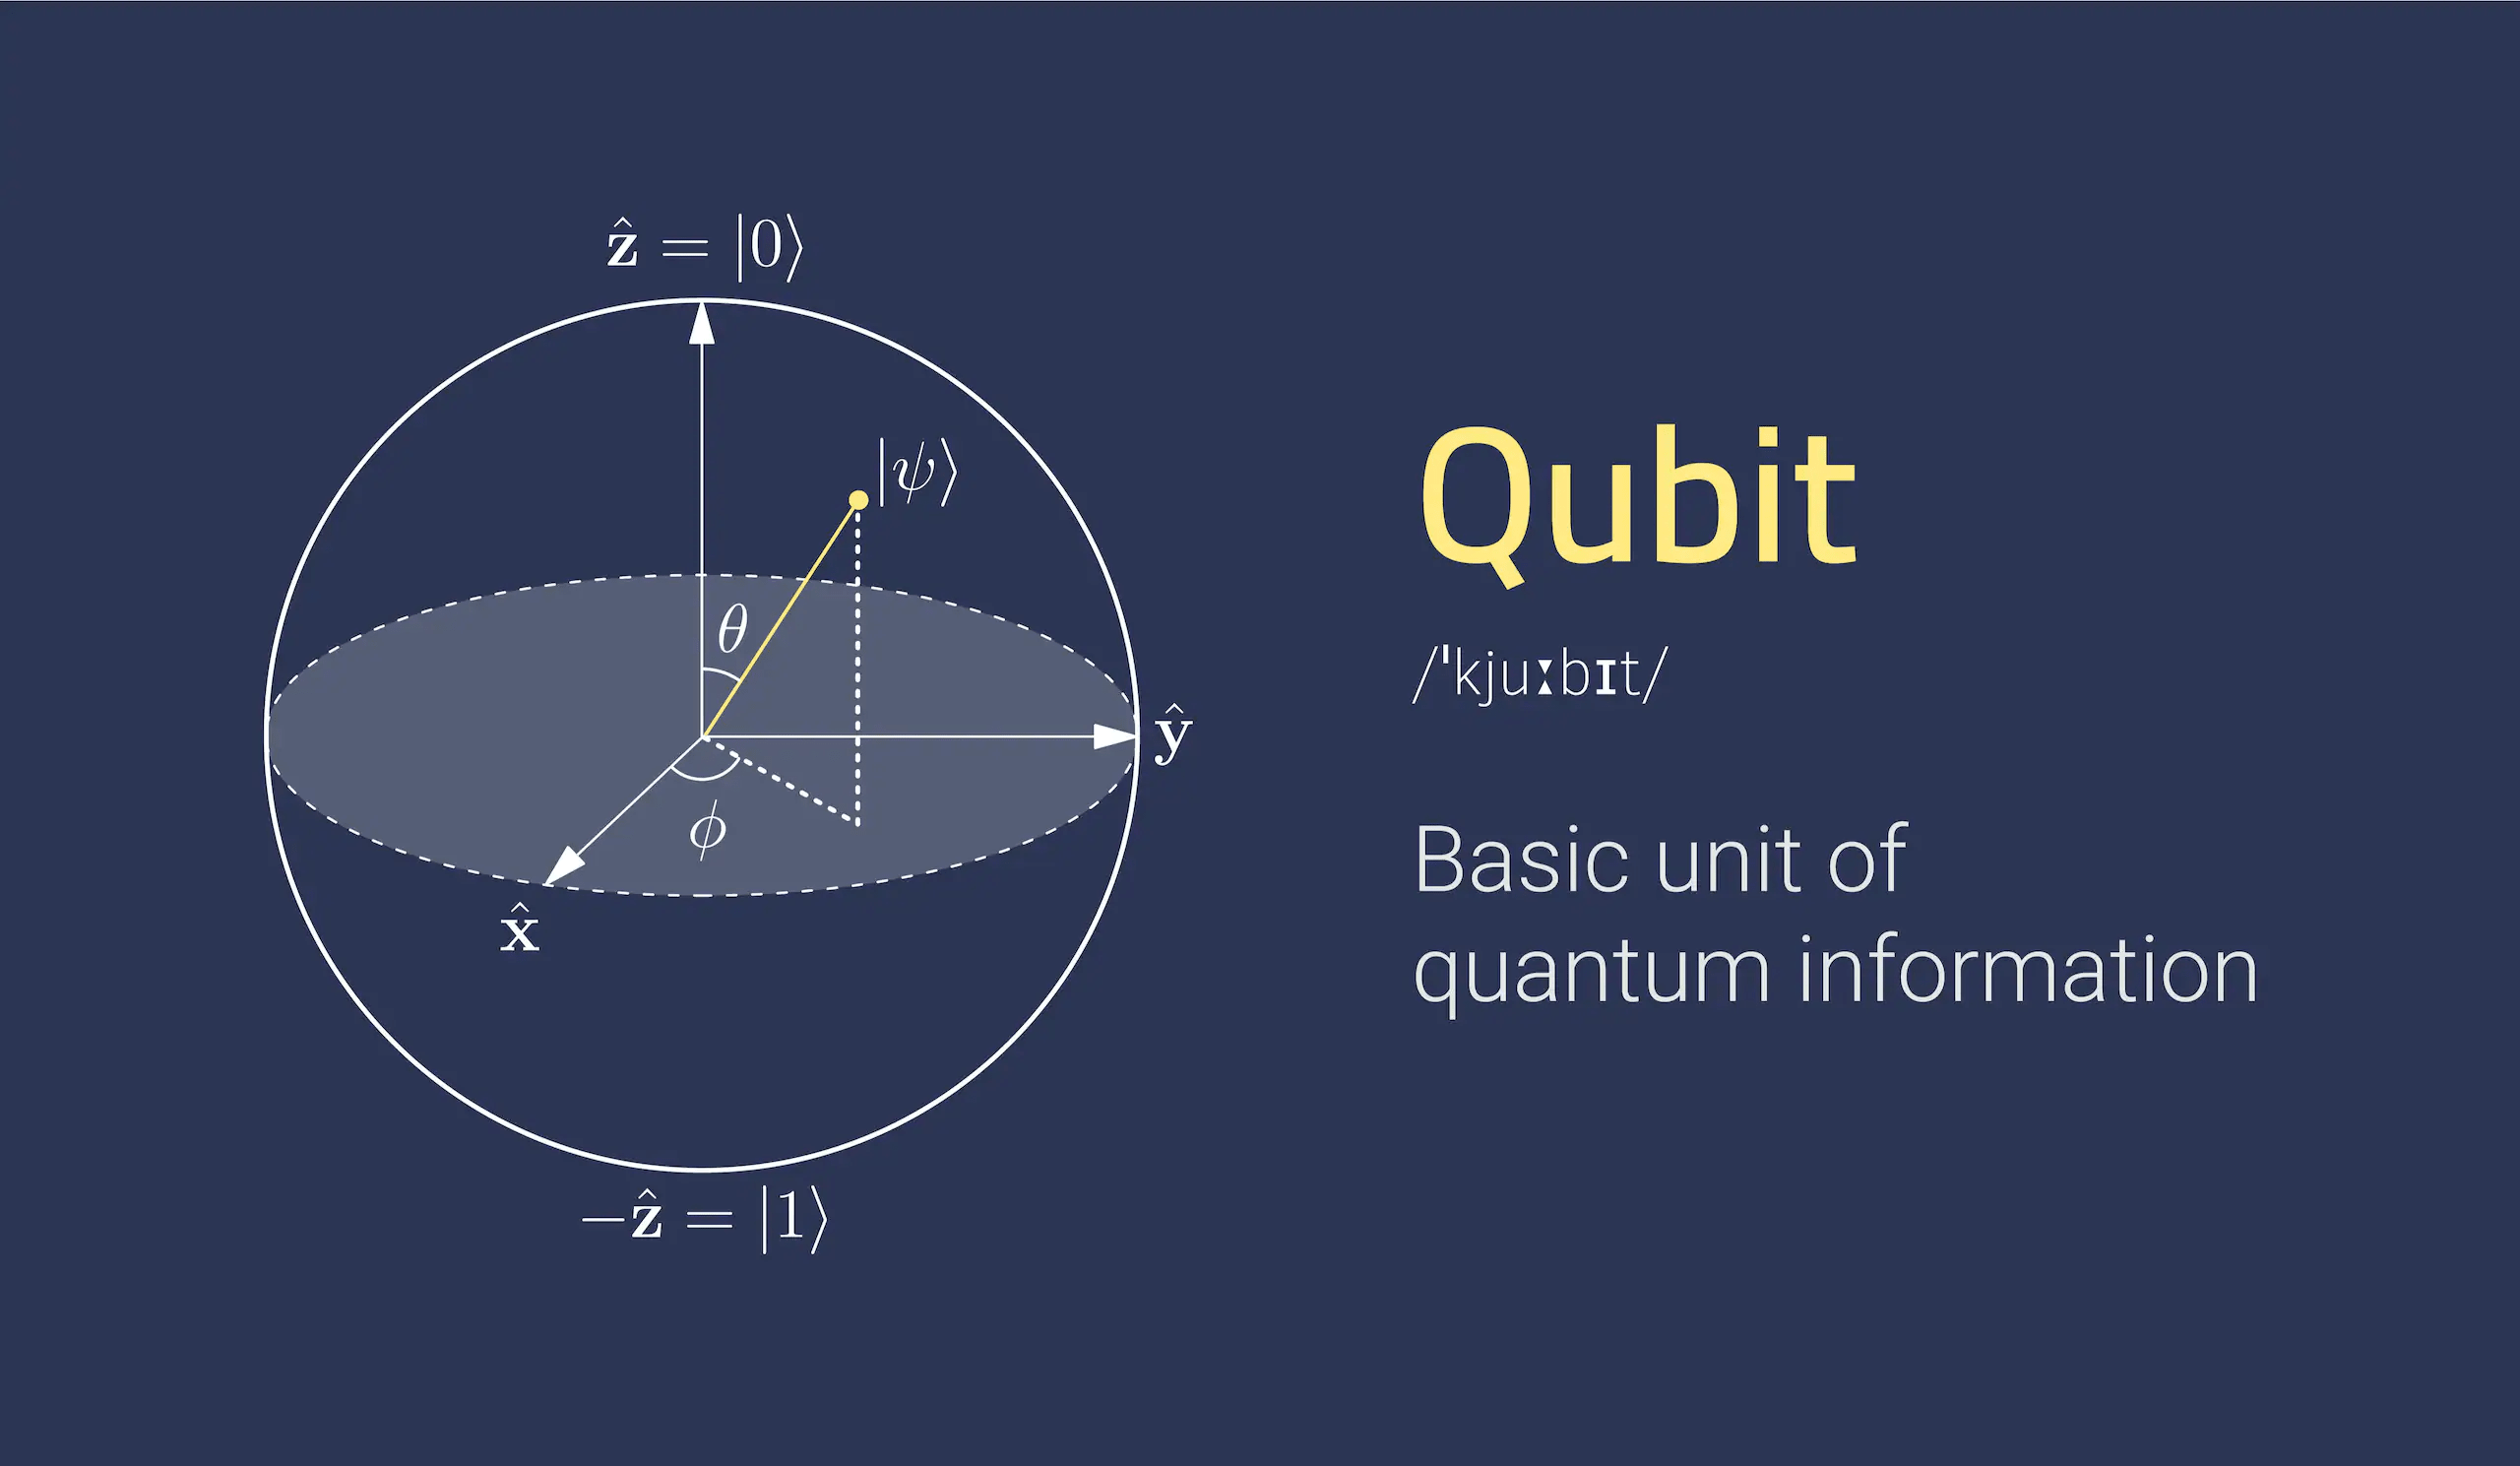
\includegraphics[keepaspectratio=true,scale=0.15]{img/qubit.png}}
\captionof{figure}{кубит}\label{SVM}%      only if needed  
\end{minipage}

~\\

Понятно, что кубит содержит в себе больше информации, чем классический бит.

Важным и уникальным свойством квантового распределения ключей является способность двух взаимодействующих пользователей обнаруживать присутствие любой третьей стороны, пытающейся получить информацию о ключе. Это является следствием фундаментального аспекта квантовой механики: процесс измерения квантовой системы в целом нарушает ее. Третья сторона, пытающаяся подслушать ключ, должна каким-то образом измерить его, тем самым создавая обнаруживаемые аномалии. Используя квантовые суперпозиции или квантовую запутанность и передавая информацию в квантовых состояниях, может быть реализована система связи, обнаруживающая подслушивание. 	

Традиционная криптография с открытым ключом , которая опирается на вычислительную сложность определенных математических функций и не может предоставить никаких математических доказательств фактической сложности обращения. В отличее от неё безопасность шифрования, использующего квантовое распределение ключей, опирается на основы квантовой механики и обладает доказанной безопасностью, основанной на теории информации, и прямой секретностью .

Главный недостаток квантового распределения ключей заключается в том, что оно обычно зависит от наличия аутентифицированного классического канала связи. В современной криптографии наличие аутентифицированного классического канала означает, что либо уже произведен обмен симметричным ключом достаточной длины, либо открытые ключи достаточного уровня безопасности. 

Квантовое распределение ключей используется только для создания и распространения ключа, а не для передачи каких-либо данных сообщения. Затем этот ключ можно использовать с любым выбранным алгоритмом шифрования для шифрования (и дешифрования) сообщения, которое затем может быть передано по стандартному каналу связи.

Итак, как мы поняли, квантовая связь включает в себя кодирование информации в квантовых состояниях (кубитах). Обычно для этих квантовых состояний используются фотоны. Квантовое распределение ключей использует определенные свойства этих квантовых состояний для обеспечения своей безопасности. Существует несколько различных подходов к квантовому распределению ключей, но их можно разделить на две основные категории в зависимости от того, какое свойство они используют.

\begin{itemize}
\item \textbf{ Протоколы на основе измерений \\} 
В отличие от классической физики, акт измерения является неотъемлемой частью квантовой механики. В общем, измерение неизвестного квантового состояния каким-то образом меняет это состояние. Это является следствием квантовой неопределенности и может быть использовано для обнаружения любого перехвата связи (что обязательно включает измерение) и, что более важно, для вычисления количества перехваченной информации.
\item \textbf{ Протоколы на основе запутывания \\ }
Квантовые состояния двух (или более) отдельных объектов могут быть связаны вместе таким образом, что они должны описываться комбинированным квантовым состоянием, а не как отдельные объекты. Это называется запутыванием и означает, что, например, измерение одного объекта влияет на другой. Если запутанная пара объектов используется совместно двумя сторонами, любой, кто перехватывает любой из них, изменяет систему в целом, показывая присутствие третьей стороны (и объем полученной информации).

\end{itemize}

\section*{Оптическая связь}

\hspace{13pt} Технология КРК уже существует и коммерчески доступна, но в настоящее время она осуществляется через оптическое волокно, а не через фотоны, свободно перемещающиеся через воздух или воду.

Совсем недавно на Канарских островах был проведен эксперимент, где впервые установили базу КРК на расстоянии 144 км, показав, что возможно иметь эту квантовую связь в свободном пространстве.

Помимо проблем, связанных с передачей фотонов через воду и свободный воздух, исследователям необходимо установить лазерную связь между передатчиком и приемником на спутниковой или бортовой платформе.

В настоящее время этим занимается команда QinetiQ North America, которая разрабатывает специализированную систему отслеживания.

Как только оптическая связь между подводной лодкой и спутником установлена, работа исследователей ITT Exelis берет верх, исследуя, как включить протокол КРК для защиты связи. Это делается с помощью фотодатчика, работающего в так называемом режиме Гейгера, что фактически означает, что он считает фотоны, приходящие с определенной поляризацией.

ПО сути, для передачи квантовой информации нужно что-то, что поляризует фотоны, поэтому квантовое состояние будет в заданном базисе, и иметь фильтр, который обнаруживает это в передатчике и приемнике.

Использовать обычные лазеры нельзя, поскольку нам нужны специальные фотонные лазеры, которые похожи на очень разбавленный лазер. Они посылают по одному фотону за раз, и каждый фотон имеет четко определенное квантовое состояние.

\section*{Технико-экономические обоснования}

\hspace{13pt} На следующем этапе программы военно-морская исследовательская лаборатория США проведет серию экспериментов, чтобы установить, насколько хорошо сохраняется квантовое состояние фотона при его прохождении через воду, чтобы проверить точность теоретического технико-экономического обоснования ITT Exelis.

Если эксперименты подтвердят теоретическую модель и исследования перейдут к следующему этапу, экспериментальный прототип может быть создан в течение пяти лет. Однако на столь радикальный новый подход влияет ряд факторов.

«Это не только научно-технический вопрос, но также связан с уровнем финансирования и политикой», - заявил Ланзагорта.

Однако, если власть имущие все же доведут дело до конца, выгоды могут быть существенными. Предлагаемая система потенциально могла бы обеспечить совершенно безопасную передачу, высочайший доступный уровень безопасности, со скоростью до 170 кбайт в секунду, что примерно в 600 раз больше пропускной способности, чем способны нынешние системы ОНЧ, легко справляясь со сложными данными, такими как видео.

Кроме того, не было бы потери эксплуатационной эффективности или скрытности для самой подводной лодки, поскольку в принципе ей не нужно было бы замедляться, оставаться на глубине менее 100 м или менять ориентацию для обмена данными.

Однако весь успех зависит от того, как путешествие в воде влияет на фотон. Самая большая проблема состоит в том, чтобы увидеть, как лучше всего послать импульсы одиночных фотонов таким образом, чтобы квантовое состояние было защищено, даже если оно проходит через воду. Нужно найти способ выполнить своего рода кодирование, такое как кодирование с исправлением ошибок, которое защищает квантовое состояние фотона, чтобы мы могли иметь больший диапазон операци.

\section*{Литература}
\begin{enumerate}
\item Stanford VLF Group: \href{https://vlfstanford.ku.edu.tr/research_topic_inlin/introduction-vlf/}{\it What is ELF/VLF Research?}
\item Naval technology (30.01.2020): \href{https://www.naval-technology.com/features/featuredeep-secret-secure-submarine-communication-on-a-quantum-level/?utm_source=Army%20Technology&utm_medium=website&utm_campaign=Must%20Read&utm_content=Image}{\it Deep secret – secure submarine communication on a quantum level}
\item Wikipedia[electronic resource] (14.12.2021): \href{https://en.wikipedia.org/wiki/Quantum_entanglement}{\it Quantum entanglement}
\item Wikipedia[electronic resource] (14.12.2021): \href{https://ru.wikipedia.org/wiki/%D0%A1%D0%B2%D0%B5%D1%80%D1%85%D0%B4%D0%BB%D0%B8%D0%BD%D0%BD%D1%8B%D0%B5_%D0%B2%D0%BE%D0%BB%D0%BD%D1%8B}{\it Сверхдлинные волны}
\item Wikipedia[electronic resource] (14.12.2021): \href{https://en.wikipedia.org/wiki/Quantum_key_distribution}{\it Quantum key distribution}
\end{enumerate}

\end{document} % конец документа